\documentclass{beamer}
\usepackage{graphicx}
\usepackage[style=authoryear-icomp]{biblatex}
\usepackage{xcolor}
\usepackage{subcaption}
\usepackage{cancel}
\usepackage{graphviz}

% BEAMER SETUP
\usetheme{CambridgeUS}
\usecolortheme{rose}
\setbeamertemplate{footline}[frame number]
\usefonttheme[onlymath]{serif}

% DEFINE COMMANDS
\newcommand{\question}[1]{\textit{\textcolor{blue}{#1}}}
\newcommand{\todo}[1]{\textit{\textcolor{red}{#1}}}
\newcommand{\citationneeded}{\textbf{\color{blue}[Citation Needed]}}
\renewcommand{\footnotesize}{\fontsize{7pt}{2pt}\selectfont}
\DeclareMathOperator*{\argmin}{arg\,min} % thin space, limits underneath in displays

% PRESENTATION METADATA
\title[]{The Motion Primitives of Motions in Microseconds}
\author[]{Pravi Samaratunga}
\institute{Boston University ECE}
\date{\today}

\addbibresource{./assets/sources.bib}

\begin{document}
\begin{frame}
   \begin{center}
       \titlepage
     
       
\includegraphics[width=0.4\textwidth]{./assets/BU_logo.png}
   \end{center}
\end{frame}

\begin{frame}{Presentation Overview}
\begin{itemize}
\item Sampling-Based Motion Planning \\
\item Motion Primitives \\
\item \textit{Motions in Microseconds} \\
\item Strengths \& Weaknesses\\
\item Future Work \\
\end{itemize}
\end{frame}

\section{Introduction}
\subsection{\textsc{sbmp}}

\begin{frame}{Sampling-Based Motion Planning}

\pause
\begin{block}{What is Sampling-Based Motion Planning (\textsc{sbmp})?}
\pause Sampling-based motion planning \textsc{sbmp} is a method of determining how a robot moves through configuration space by sampling values from that space. %list off examples of algorithms, note tree-based vs graph-based
\end{block}

\pause
\begin{block}{Why is it relevant?} 
\pause \textsc{sbmp} algorithms are widely applicable and used in many fields. %list them off here
However, it can take several seconds for \textsc{sbmp} methods to execute, so there is ample space for innovation.
\end{block}

\pause
\begin{block}{How do we optimize \textsc{sbmp}?}
Over the years, many optimizations have been introduced to \textsc{sbmp}. We will discuss \textsc{vamp}, the Vector-Accelerated Motion Planning system as introduced by \cite{paper:MiM}.
\end{block}
\end{frame}

\begin{frame}{Example \textsc{sbmp} Execution: Problem Definition}
%\only<1>{Problem Definition}\only<2>{Step 1: Sample State Space}\only<3>{Step 2: Connect State to Graph}\only<4>{Step 3: Graph Search}
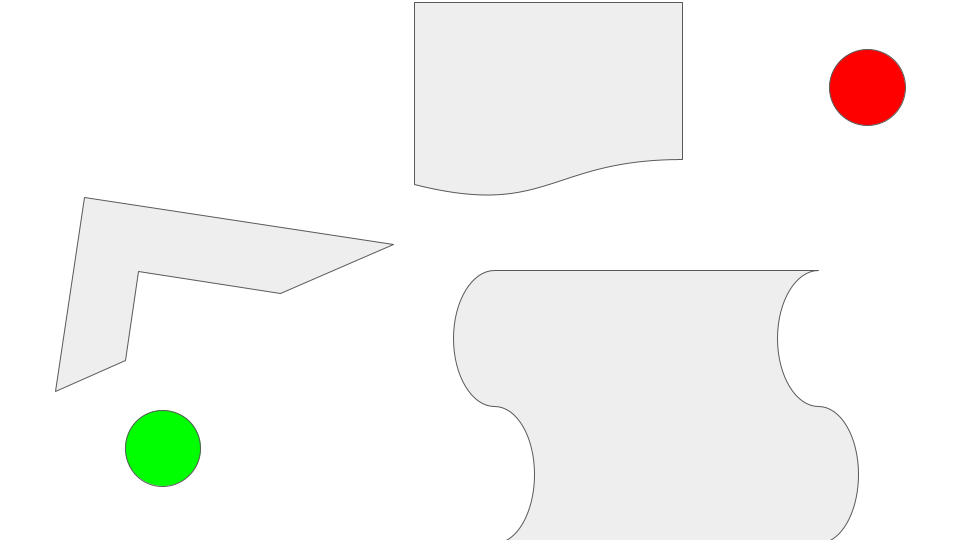
\includegraphics[width=\textwidth]{./assets/rrt_slides/rrt_slides_2.png}
\end{frame}

\begin{frame}{Example \textsc{sbmp} Execution: Sampling}
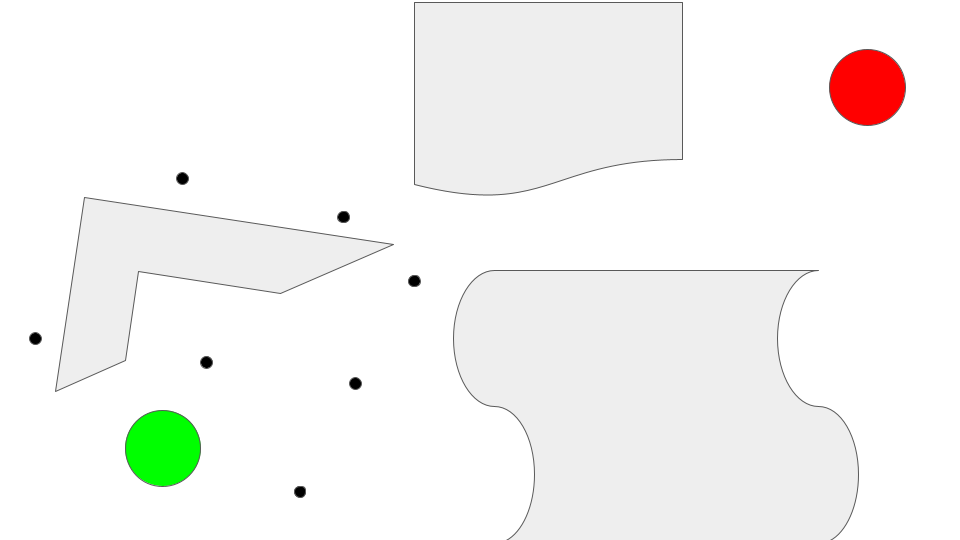
\includegraphics[width=\textwidth]{./assets/rrt_slides/rrt_slides_3.png}
\end{frame}

\begin{frame}{Example \textsc{sbmp} Execution: Local Planning}
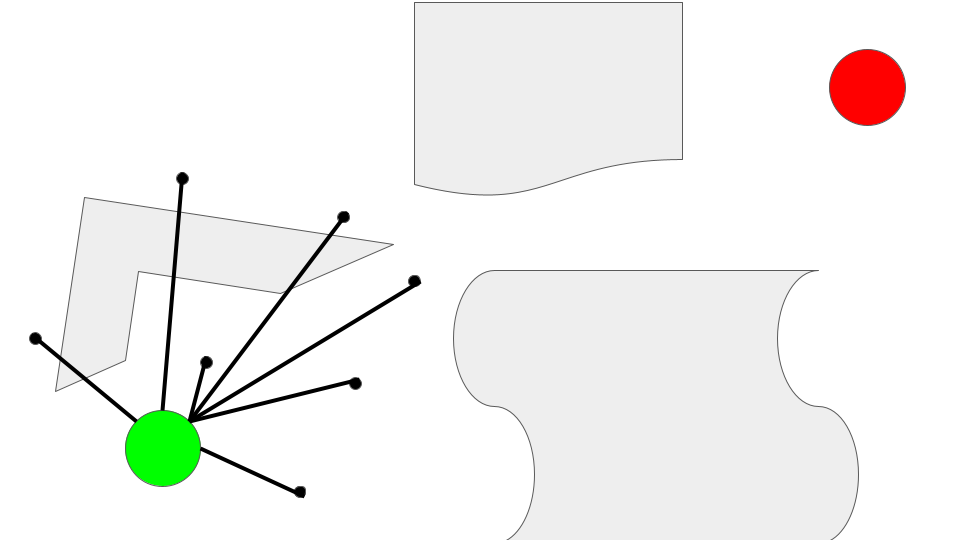
\includegraphics[width=\textwidth]{./assets/rrt_slides/rrt_slides_4.png}
\end{frame}

\begin{frame}{Example \textsc{sbmp} Execution: Collision Checking}
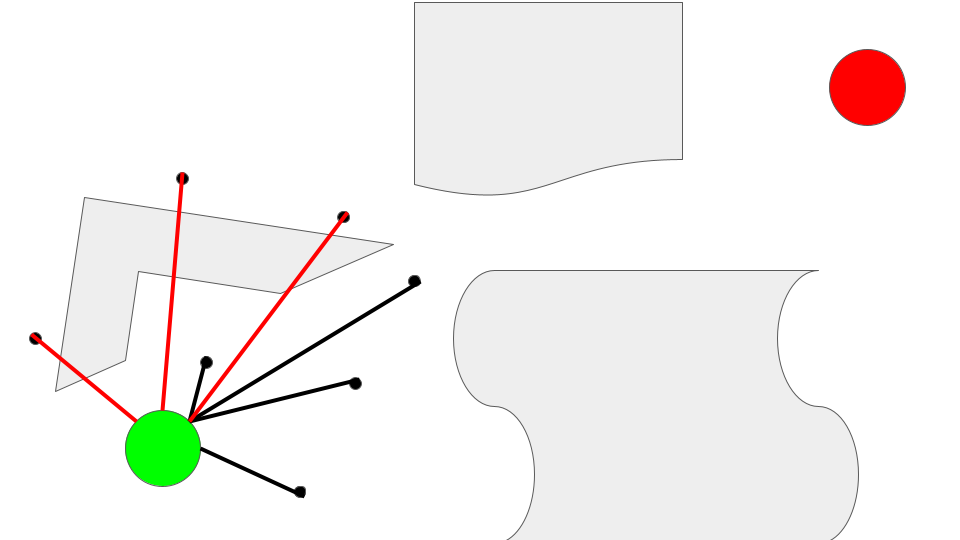
\includegraphics[width=\textwidth]{./assets/rrt_slides/rrt_slides_5.png}
\end{frame}

\begin{frame}{Example \textsc{sbmp} Execution: Motion Validation}
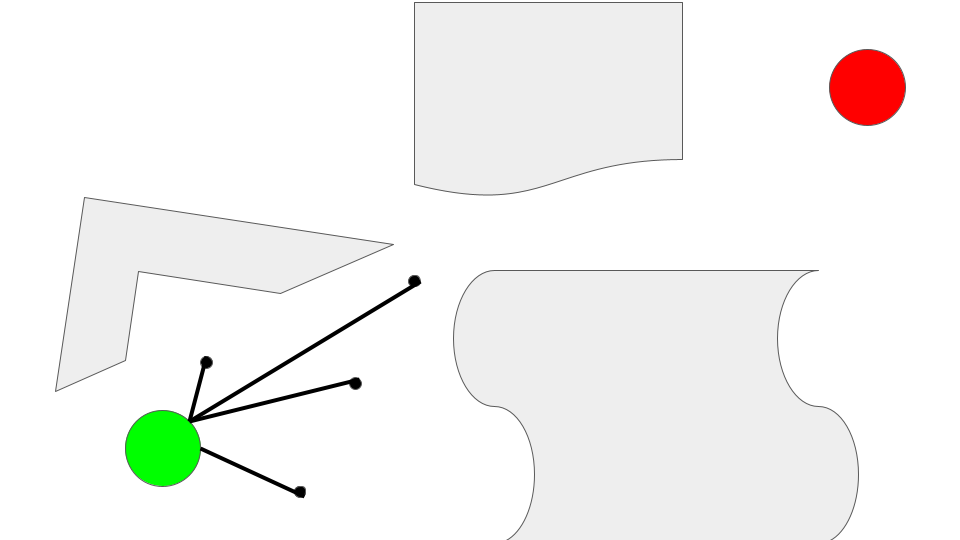
\includegraphics[width=\textwidth]{./assets/rrt_slides/rrt_slides_6.png}
\end{frame}

\begin{frame}{Example \textsc{sbmp} Execution: Generate Whole Graph}
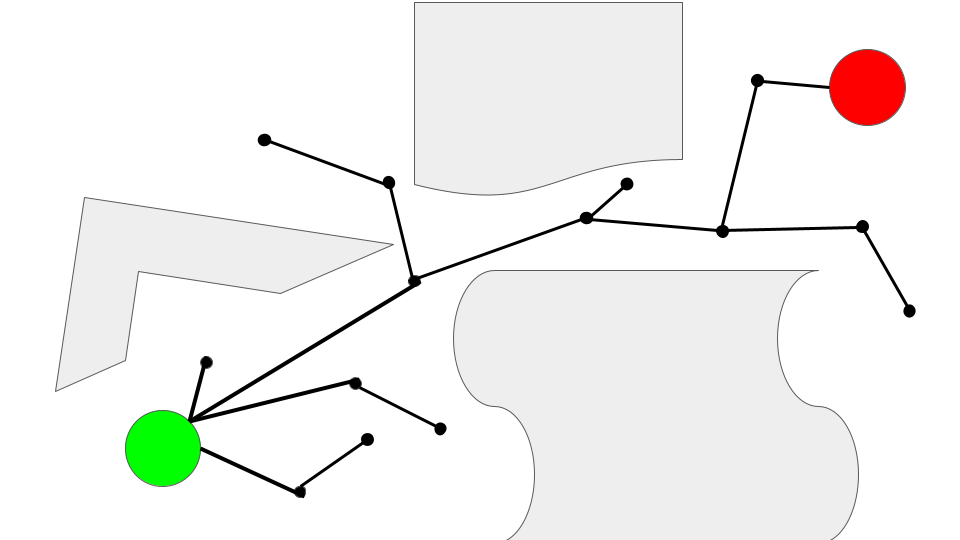
\includegraphics[width=\textwidth]{./assets/rrt_slides/rrt_slides_7.png}
\end{frame}

\begin{frame}{Example \textsc{sbmp} Execution: Find Path}
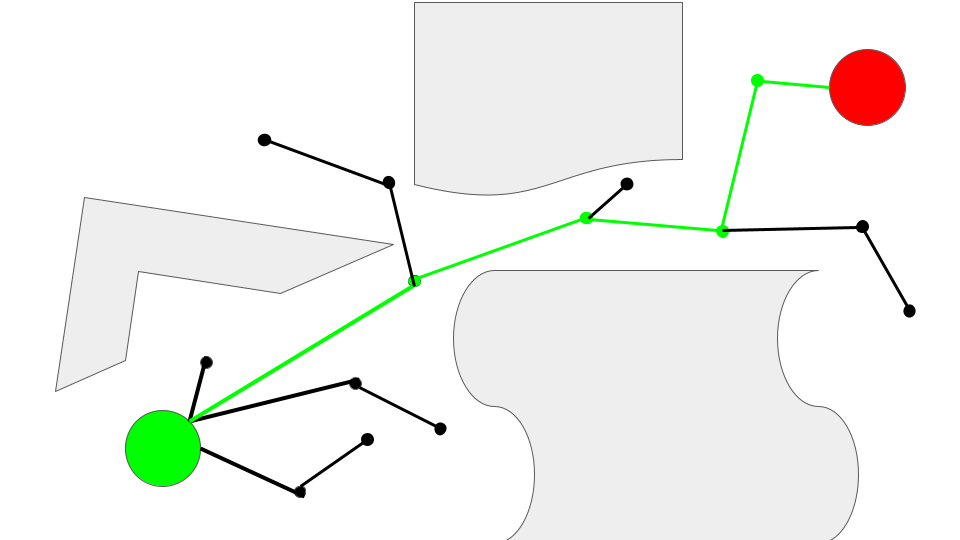
\includegraphics[width=\textwidth]{./assets/rrt_slides/rrt_slides_8.png}
\end{frame}

\subsection{Planning Primitives}

\begin{frame}{Planning Primitives}
% Having gone over the shape of RRT, let's identify what common primitives happen across many sampling-based motion planners.
\pause
\begin{block}{Nearest Neighbors Search (\textsc{nn})}
Part of the sampling function for the state space.
\end{block}

\begin{block}{Forward Kinematics (\textsc{fk})}
Maps configuration-space elements to physical space.
\end{block}

\begin{block}{Collision Checking (\textsc{cc})}
Ensures that obstacles do not collide with the robot. Uses many passes of \textsc{fk} in computation. 
\end{block}

\textsc{cc} is conventionally thought of as the most computationally intensive step of the motion planning process.%, so much of the discussion is in optimizing \textsc{cc} and \textsc{fk}

\end{frame}

\begin{frame}
\centering
\textbf{How do we optimize these computationally intensive tasks?}
\end{frame}

\subsection{State of the Art}

\begin{frame}
\textsc{fk} computations are difficult to parallelize due to the robot geometry introducing data dependencies.

In order to minimize the total number of \textsc{cc} calls, it is often performed in two steps, \textit{broadphase} and \textit{narrowphase}. \cite{paper:eemp} developed a method for using local sparsity patterns in a parallel manner.
\end{frame}

\section{Motions in Microseconds}

\subsection{\textsc{vamp}}

%\cite{paper:MiM} presents Vector-Accelerated Motion Planning (\textsc{vamp}).

\begin{frame}{Vectorizing Motion Planning}
\pause
\begin{block}{Vector}
A \textit{vector} is a fixed-length sequence of scalar values.
\end{block}

\begin{block}{Vectorized Operation}
A \textit{vectorized operation} acts on all values within the vector. This operation must be done independently, in parallel.
\end{block}

\pause
\cite{paper:MiM} chose to focus on CPU-level parallelism, rather than GPU-level, process-level, or thread-level parallelism, so as to incur less overhead.
\end{frame}

\begin{frame}{Vector Accelerated Motion Planning (\textsc{vamp})}
\pause
\textsc{vamp}'s innovations over State of the Art:
\begin{itemize}
\item Struct-of-Arrays data representation
\item Tracing Compiler
\item Geometric Intersection Tests
\item Raked Motion Validator implementation
\end{itemize}
\end{frame}

\begin{frame}{Struct-of-Arrays}
%The more intuitive data representation is AoS, but
\centering
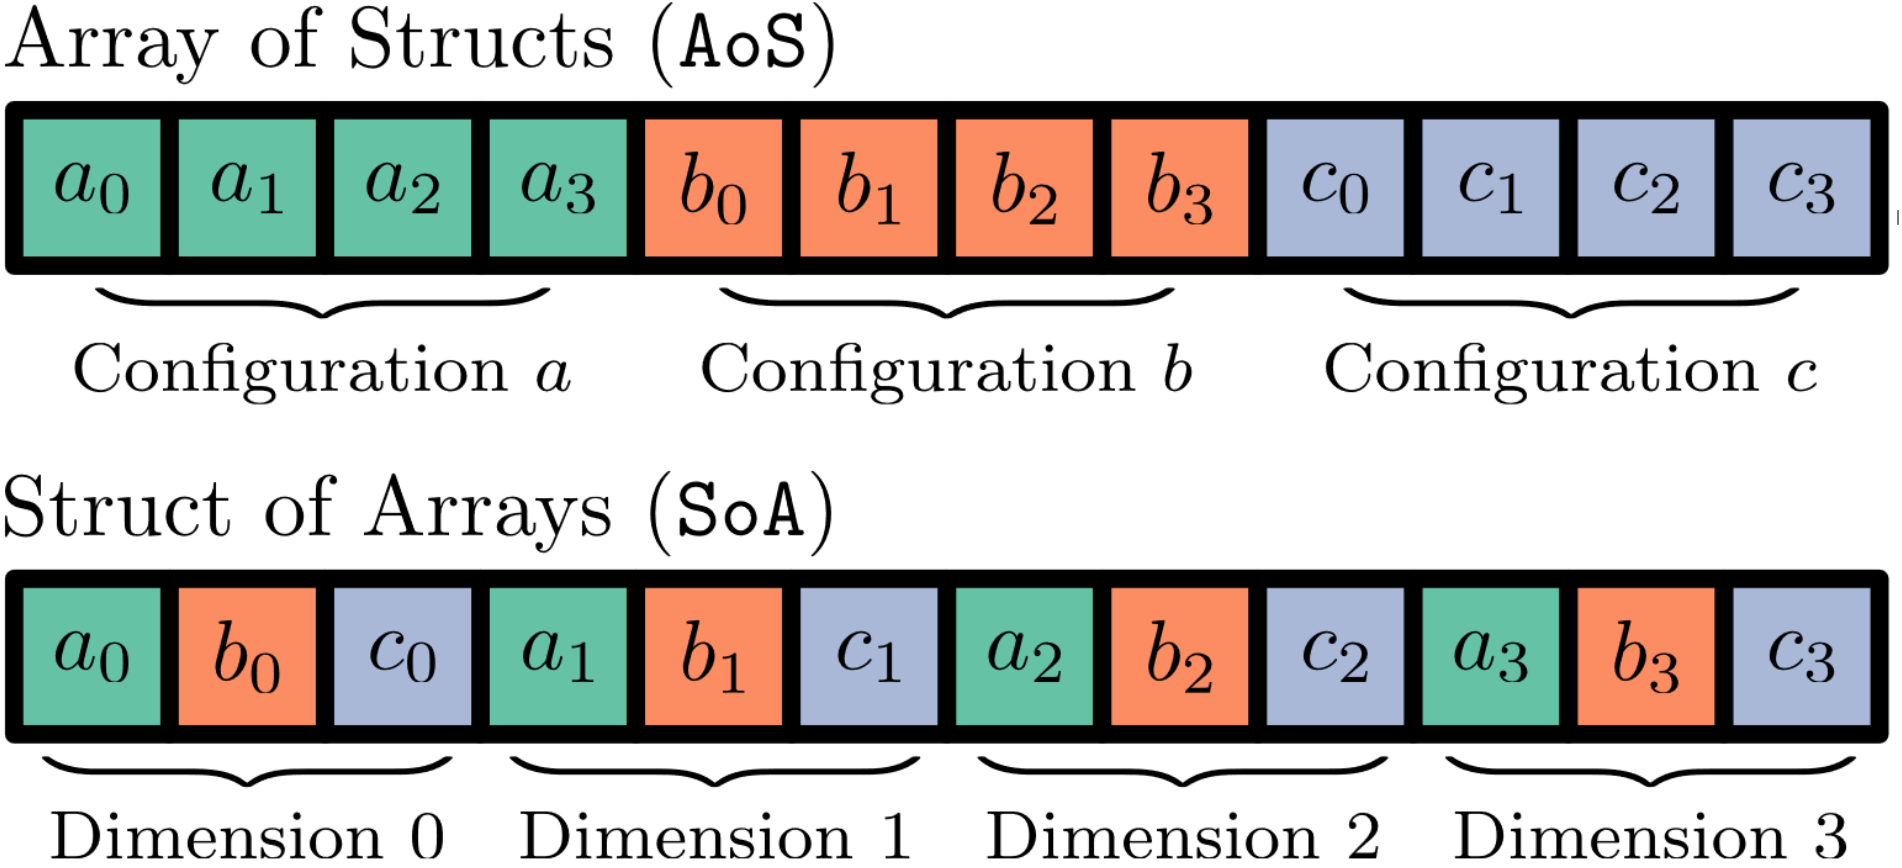
\includegraphics[width=\textwidth]{./assets/soa_aos.png}
\end{frame}

\begin{frame}{Tracing Compiler}
%\textsc{fk} has been difficult to parallelize with prior approaches due to data dependencies between link transforms in the kinematic chain.
To vectorize \textsc{fk}:
\begin{itemize}
\item Trace the operations of the robot's kinematics from a \textsc{urdf} file.
\item Generate a vector configuration structure for a batch of configurations. 
\item Output a minimal set of operations to compute the traced function as an unrolled loop.
\end{itemize}

Notably, this tracing technique generates optimized \textsc{fk} implementations at compile time through automatic code generation.
\end{frame}

\begin{frame}{Geometric Intersection Tests}
\begin{columns}
\begin{column}{0.5\textwidth}
By representing the robot as a system of geometric objects, intersection tests between pairs of objects can be vectorized.

\vspace{10px}

This approach does away with the staged broadphase and narrowphase approach to collision checking, but focuses soley on narrowphase.
\end{column}
\begin{column}{0.5\textwidth}
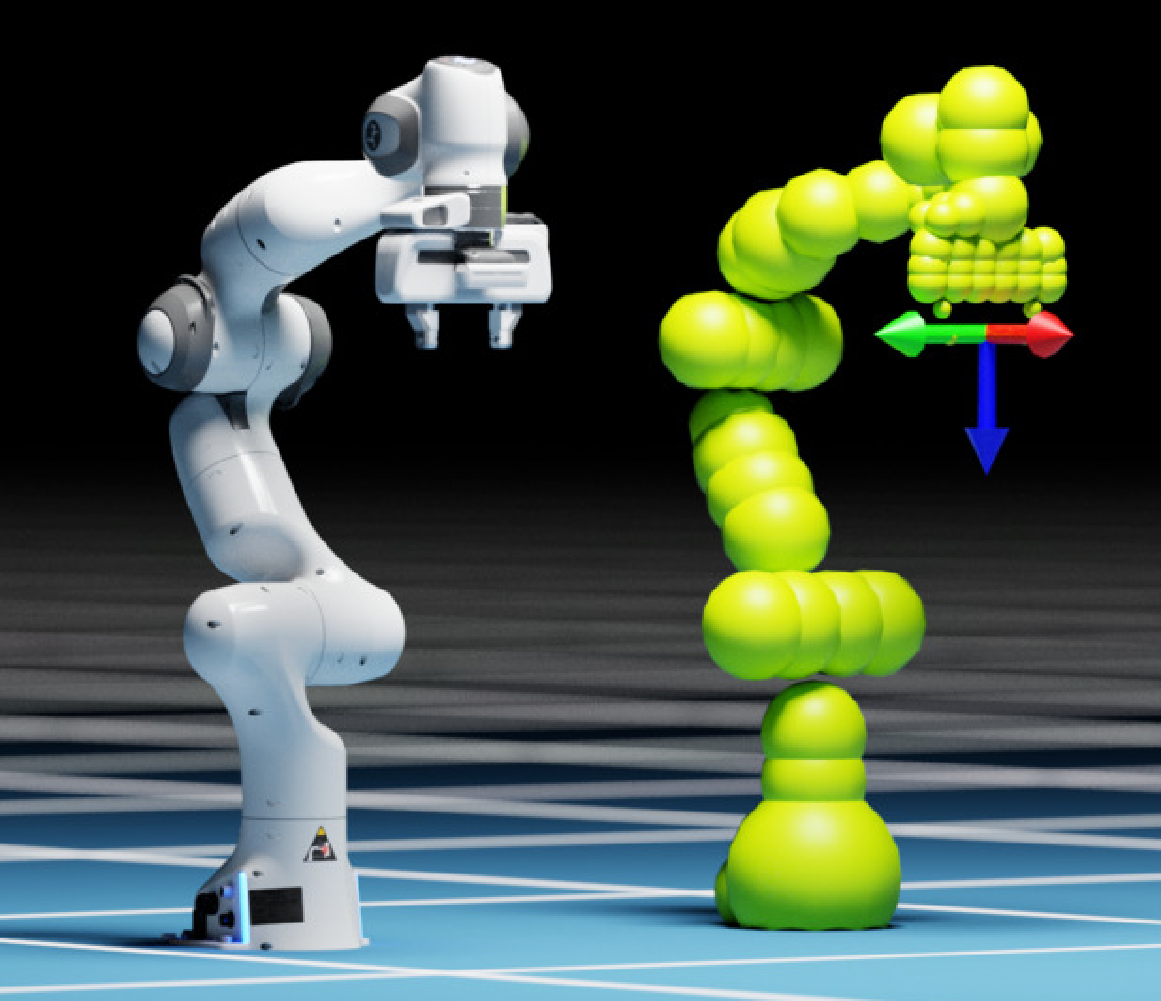
\includegraphics[width=\textwidth]{./assets/panda_spheres.png}
\end{column}
\end{columns}
\end{frame}

\begin{frame}{Raked Motion Validator Implementation}
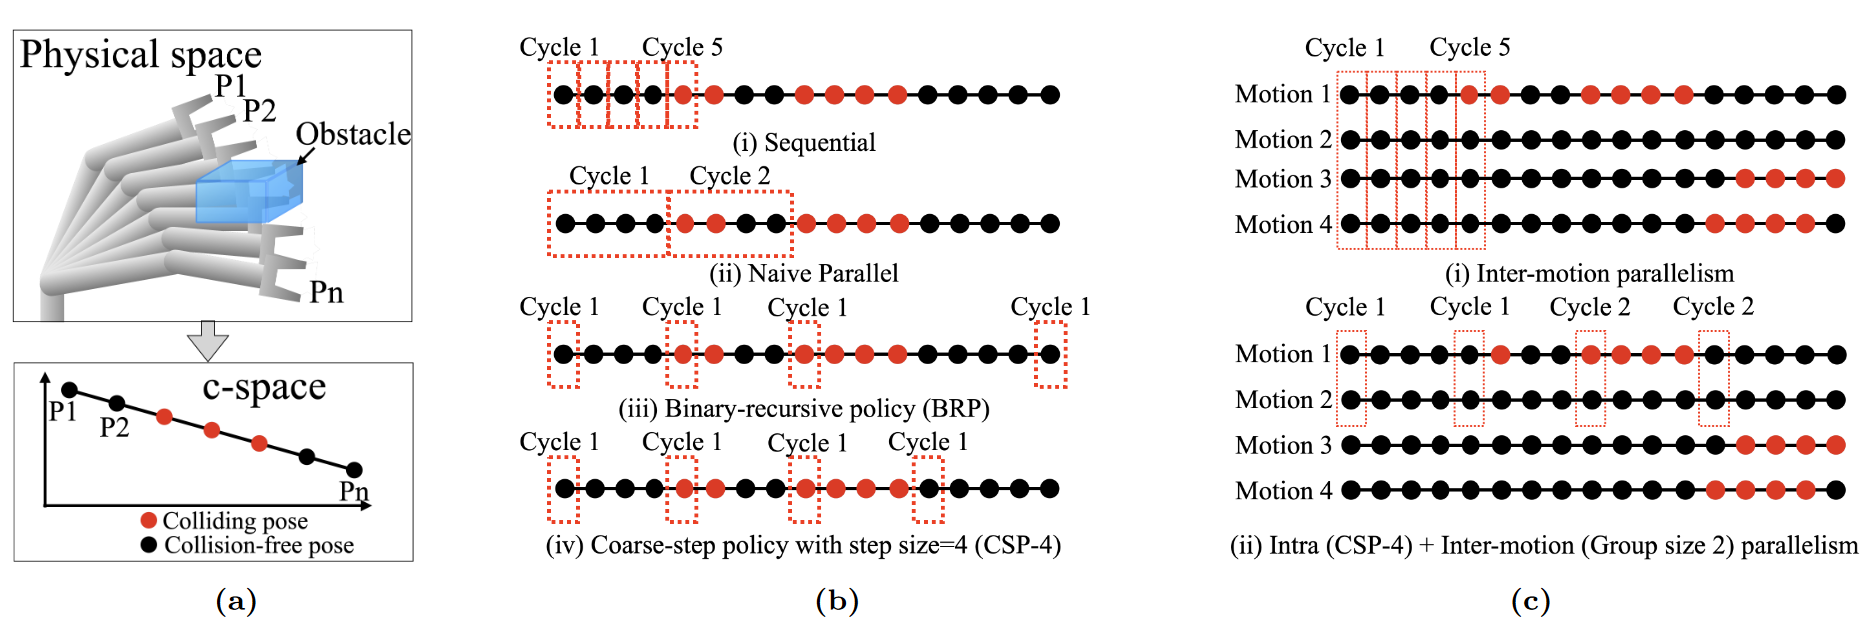
\includegraphics[width=\textwidth]{./assets/eemp_mv.png}

[\cite{paper:eemp}]
\end{frame}

\section{Strengths \& Weaknesses}

\subsection{Strengths}

\begin{frame}{Strengths}
With straightforward architechtural optimizations, the authors get upwards of 500$\times$ speedups over PyBullet, and 100-200$\times$ over MoveIt, both using \textsc{ompl} for the motion planning implementation.

%The authors made innovations that no one before them realized would matter so significantly.
\end{frame}

\begin{frame}{Weaknesses}
The authors don't consider end-to-end performance impacts. \todo{it's too late. include table?}

\todo{What difference does the 7DOF vs 8DOF robot make?}
\end{frame}

\section{Future Work}

\begin{frame}{Future Work}
\todo{polish, format, beef up}

\begin{itemize}
\item exploit structured information about manipulator \& environment
\item explore non-sphere geometric representations of colliders (eg trimeshes, capsules)
\end{itemize}
\end{frame}

\section {TODO}

\begin{frame}
\todo{Things to improve
\begin{enumerate}
\item Future Work
\item Strengths \& Weaknesses
\item Figures post-presentation
\item explanation of raked mv
\end{enumerate}}
\end{frame}
\end{document}